\subsubsection{Hipótesis}

Para este filtro en particular, dada su complejidad, en cuanto al orden necesario para acceder en memoria a los valores, y los calculos para arrivar al resultado, hipotetizamos que la diferencia obtenida entre la mejor version de ASM y la mejor version de C serian mayores que las mismas comparaciones entre otros filtros, debido a que las optimizaciones que el compilador pudiese efectuar sobre el codigo y los accesos a memoria, no serian tan buenas como hacer un analisis especifico del funcionamiento del filtro y deduciendo que valores se puede reutilizar y que calculos se pueden realizar en paralelo utilizando instrucciones SSE.

Por otro lado realizamos 2 versiones diferentes tanto en C como en ASM con la idea de poder comparar por un lado la ganancia posible a travez de instrucciones SSE y por otro la gananica de reordenar la forma de acceso a los datos.


\subsubsection{Resultados obtenidos}


Los resultados que obtuvimos estuvieron razonablemente dentro de lo esperado. La ganancia entre la mejor version de ASM y la mejor de C con optimizacion en O3, permitiria aplicar el filtro en un poco mas de 4 imagens al mismo tiempo que la de C se lo aplica a 1 sola, o tambien, pudiendo aplicar el filtro a una imagen del doble de ancho y doble de alto (lo cual es muy util en el contexto de pantallas cada vez con mas resolucion). 

Tambien de alguna manera esperado fue que la ganancia utilizando SIMD fuese de ~4x dado que es justamente la cantidad de pixels que se pueden manejar simultaneamnte .

\begin{table}[!htbp]
	\centering
	\footnotesize
	\begin{tabular}{| c | c | c | c | c | c |}
		\hline
Pixels & ASM & C (o3) & C preproc (o3) & ASM simd & ASM simd preproc \\ \hline
16x16  & 33357 & 18596 & 13153 & 5194 & 3449 \\ \hline
32x32  & 181961 & 101292 & 62862 & 27944 & 15221 \\ \hline
64x64  & 837330 & 465902 & 289280 & 134856 & 65339 \\ \hline
128x128  & 3574572 & 1995407 & 1231802 & 548901 & 272744 \\ \hline
256x256  & 14911141 & 8238530 & 5276382 & 2274634 & 1159197 \\ \hline
512x512  & 61337662 & 34614421 & 22898444 & 9514187 & 4865965 \\ \hline
1024x1024  & 246805935 & 135432773 & 85989437 & 38506702 & 20900364 \\ \hline
2048x2048  & 996559614 & 547159461 & 348591233 & 156452341 & 90032611 \\ \hline
4096x4096  & 4139577580 & 2273534155 & 1566227645 & 639810532 & 363950690 \\ \hline
8192x8192  & 16999317092 & 9493848236 & 6354314134 & 2644797660 & 1533749148 \\ \hline
Relacion & 11.0835054834 & 6.1899615386 & 4.1429944018 & 1.7244004102 & 1 \\ \hline

	\end{tabular}
\end{table}


\begin{figure}[!h]
	\centering
	\begin{minipage}{.5\textwidth}
		\centering
		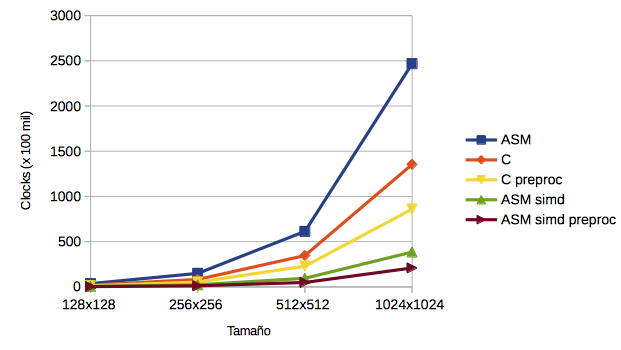
\includegraphics[width=\linewidth]{imgs/ldrTotales1.png}
	\end{minipage}\hfill
	\begin{minipage}{.5\textwidth}
		\centering
		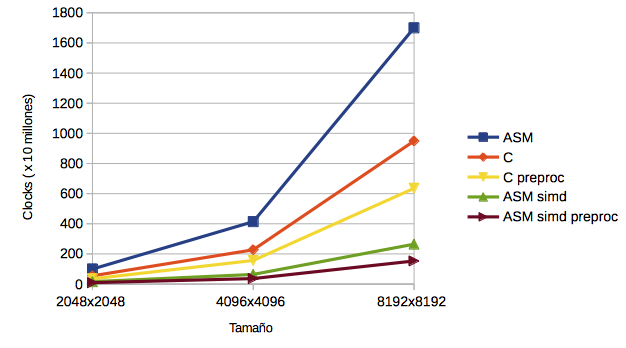
\includegraphics[width=\linewidth]{imgs/ldrTotales2.png}
	\end{minipage}\hfill
\end{figure}
 

\newpage

A su vez pudimos observar el poder de la optimizacion de C, ya que sin ningun esfuerzo de parte del programdor se obtiene una ganacia muy interesante, sobrepazando inclusive la version realizada en asm que no utilizaba instrucciones de SIMD.


\begin{figure}[!h]
	\centering
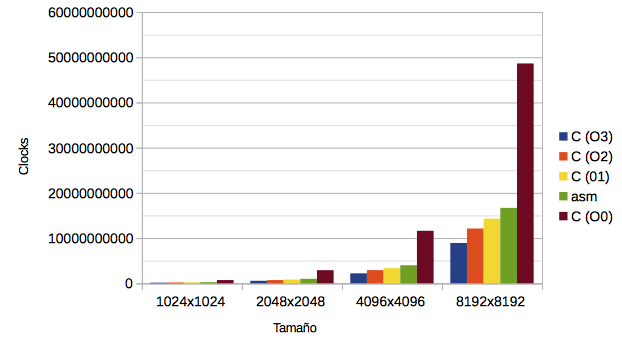
\includegraphics[width=300px]{imgs/ldrOptC.png}
\end{figure}




Dentro de los experimentos que decidimos realizar, nos preguntamos si existiria alguna diferencia en el el tiempo utilizado por los algoritmos dependiendo del parametro alpha, dado que se utiliza para multiplicar cada pixel.
Es interesante ver como se ve en el resultado de esta imagen, que para el valor de alpha=0, la cantidad de clocks utilizado, por los algoritmos que utilizan floats para la multiplicacion, diminuye significativamente. 
De esto se pueden sacar varias conclusiones interesantes, por un lado que la multiplicacion por el alpha consume una parte muy importante del tiempo total utilizado por el algoritmo.
Que si el valor es 0, el procesador resuelve inmediatamente el resultado y ademas que para el resto de los valores, no hay diferencia segun el valor por el cual se multiplique.

\begin{figure}[!h]
	\centering
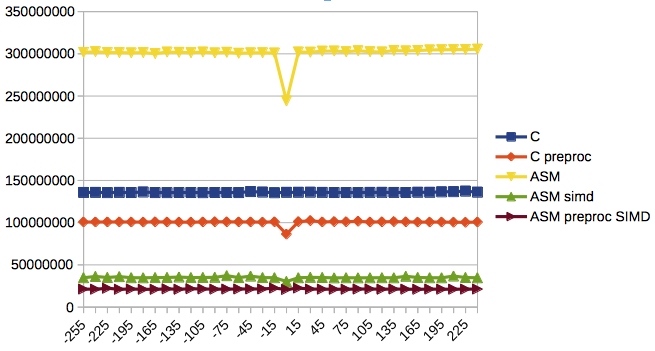
\includegraphics[width=300px]{imgs/comparacionLDR.png}
\end{figure}

